
%\chapter{Faster Search for Merging Candidates} \label{chp:metrics}
\chapter{Faster Function Merging} \label{chp:fastfm}


%In this chapter, we will focus on the sequence alignment algorithm and the search for merging candidates.


Contributions:
- HyFM is the first function merging technique capable of merging code regardless of the basic block ordering.

\section{Motivation}


In this section, we show how the different stages of the optimisation process can impact on the compilation time, depending on the program being compiled.
%In this section, we show how different programs spend  more time on different stages of the optimisation process.
For programs with large number of functions, the time spent searching for merging candidates may be considerable relative to the other stages.
The search strategy described in Chapter~\cite{chp:cgo19} uses a fingerprint-based ranking approach where for each function, all other candidate functions are ranked based on the distance between fingerprints.

\begin{figure}[h]
  \centering
  \includegraphics[width=0.95\textwidth]{src/fastfm/figs/compilation-breakdown-motivation-ranking.pdf}
  \caption{.}
  \label{fig:compilation-breakdown-motivation}
\end{figure}

%%TODO: specify the number of functions in each the benchmarks used as example

\begin{figure}[h]
  \centering
  \includegraphics[width=0.95\textwidth]{src/fastfm/figs/compilation-breakdown-motivation-alignment.pdf}
  \caption{.}
  \label{fig:compilation-breakdown-motivation-alignment}
\end{figure}


For programs with very large functions, the time spent merging functions searching may dominate the compilation time.
More specifically, the time required for performing sequence alignment.
When merging two functions, the goal is to identify which segments of the code are equivalent (and therefore can be merged) and which ones are different.
To this end, SalSSA uses an optimal sequence alignment algorithm, called the Needleman-Wunsch algorithm, which is quadratic on the size of the input sequences.
Since SalSSA applies it on the linearised sequences of the whole input functions, the time spend aligning sequences can be significant for programs with very large functions.

Figure~\ref{fig:compilation-breakdown-motivation-alignment} shows two programs, from SPEC 2017, for which the time spent on sequence alignment dominates the overall running time of the function merging optimisation.
Our experiments show that SalSSA can spend up to 85\% of the time performing sequence alignment for programs such as \texttt{602.gcc\_s} and \texttt{638.imagick\_s} from SPEC 2017, with a total of 15454 and 2457 functions, respectively.
The largest functions in these two programs have 73127 and 28974 instructions, respectively.


% benchmark,      num functions, largest function 
% 602.gcc_s,      15454,         73127
% 638.imagick_s,  2457,          28974


The function merging technique proposed by von Koch~et~al.~\cite{edler10} restricts merging to nearly identical functions.
They only allow for pairs of corresponding instruction to differ, as long as they still have equivalent data type, where a diamond-shape branch is created to select which instruction will be executed depending on a function identifier.
A phi-node is used to unify the mismatching instructions as a single named value.
Every use of the mismatching instructions will refer to their phi-node.
Two instructions match if they have the same opcode with equivalent data types and operands.
Note that no operand selection is performed.
Even if two instructions differ only on their operands, they are classified as mismatching, and a branch is created.

\begin{figure}[h]
  \centering
  \includegraphics[width=0.98\textwidth]{src/fastfm/figs/soa-example-1.pdf}
  \caption{.}
  \label{fig:soa-example-1}
\end{figure}

Except for mismatching pairs of instructions, the two functions must have identical function types, i.e., they must have the same return type and list of arguments, identical CFGs, with corresponding basic blocks having the same number of instructions.

** however, these instructions must define names representing the same data type.

\begin{figure}[h]
  \centering
  \includegraphics[scale=0.9]{src/fastfm/figs/soa-example-2.pdf}
  \caption{.}
  \label{fig:soa-example-2}
\end{figure}



\section{Contributions}

In this section, we present our new function merging strategy, called HyFM, which is a hybrid between SalSSA and the technique proposed by von Koch~et~al.
Our goal is to design a technique with powerful merging capabilities while still being fast, resulting in low compilation time overheads.
This would allow us to apply function merging on much larger programs, without significantly degrading compilation time.



The function merging pass involves three major steps:
the merge operation that produces a merged function for a given pair of input functions;
the search strategy responsible for deciding which pairs of functions are worth attempting to merge;
finally, a profitability analysis that decides whether a merged function reduces code size and therefore should be kept, otherwise, the original input functions are kept unmodified.
In this chapter, we focus on the two major steps, while using the same profitability analysis presented in Chapter~\ref{chp:cgo19}.

%HyFM has an overall architecture similar to SalSSA (and FMSA).
%Similar to SalSSA, HyFM also works on any two arbitrary functions.

%, even when they have few similarities and merging them would be counter-productive.

%In the best case, the two input functions are identical and the result is equivalent to simply using one of the functions.
%In the worst case, the two input functions have no similarity and the merged function has just one entry point that branches to the correct function, depending on the function identifier.
%HyFM creates an if-else structure around both input functions.

%For that reason, we also introduce a cost model to decide
%when it is beneficial to merge two functions (see Section~\ref{sec:profit-model}).
%To avoid an expensive quadratic exploration, we integrate our profitability analysis
%with an efficient ranking mechanism based on a lightweight fingerprint of the functions.

Figure~\ref{fig:func-merge-opt-arch} shows the overall architecture of our new function merging technique.

\begin{figure}[h]
  \centering
  \includegraphics[scale=0.85]{src/fastfm/figs/func-merge-opt-arch.pdf}
  \caption{.}
  \label{fig:func-merge-opt-arch}
\end{figure}

\subsection{Search Strategy}

In this section, we give an overview of the search strategy proposed by HyFM, describing how it improves over the strategy from FMSA and SalSSA.
The purpose of the search strategy is to pair similar functions for merging but avoiding a prohibitively expensive quadratic number of merging attempts.
The purpose of the search strategy is to avoid a quadratic exploration that attempts to merge all possible pairs of functions.
%which is the same strategy used by our prior work, i.e., FMSA and SalSSA.
All three techniques use a ranking strategy based on the \textit{fingerprint} of the functions to evaluate their similarity.
They start by precomputing and caching fingerprints for all functions.
%The purpose of the fingerprints is to make it easy to discard unpromising pairs of functions so that we perform the more expensive evaluation only on the most promising pairs.
The fingerprint is a fixed-size vector that summarises the content of the function.
To this end, the fingerprint consists of a map of instruction opcodes to their frequency in the function.
While functions can have several thousands of instructions, an IR usually has just a few tens of opcodes, e.g., the LLVM IR has only about 68 different opcodes.
%This means that the fingerprint needs to store just a small integer array of the opcode frequencies.

The fingerprint representation allows us to compare functions using a simple distance metric, such as the Manhattan distance.
Figure~\ref{fig:hyfm-ranking} illustrates this search strategy.
For a given reference function, all other functions are ranked based on the distance of their fingerprints.
The candidate function with the smallest distance will be used for a merging attempt.

%By comparing the opcode frequencies of two functions, we are able to estimate
%the best case merge, which would happen if all instructions with the same opcode could match.
%This is a very optimistic estimation. It would be possible only if instruction types and order
%did not matter. We refine it further by estimating another best case merge, this time based
%on type frequencies, which would happen if all instructions with the same data type could match.

\begin{figure}[h]
  \centering
  \includegraphics[scale=0.8]{src/fastfm/figs/hyfm-ranking.pdf}
  \caption{.}
  \label{fig:hyfm-ranking}
\end{figure}

Even though computing the distance between two fingerprints is significantly faster than merging two functions, ranking can still take a considerable portion of the compilation time for program with a large number of functions.
The ranking, as implemented by FMSA and SalSSA, still requires a quadratic number of fingerprint comparisons.
HyFM limits the ranking impact on compilation time by setting a maximum number of fingerprint comparisons per reference function.
Ideally, the function with shortest fingerprint distance would be the first candidate function in the list of candidates.
To this end, HyFM sorts the list of available functions so that close by functions tend to have similar fingerprints.
Figure~\ref{} shows how different comparison methods affect the position of the functions with most fingerprint similarities.

\subsection{Merging Two Functions}


\subsubsection{Greedy Sequence Alignment}

Since HyFM merges the instructions between two basic blocks in a pairwise manner, they must have the same number of instructions.
This restriction can be leveraged to narrow down the search space.
Figure~\ref{fig:hyfm-alignment-1} illustrates this process.
First, for one of the input functions, we group all its blocks by their number of instructions, excluding phi-nodes.
%These encodings allow us to quickly search for matching candidate blocks since they would have identical encodings.
Then, HyFM iterates over all blocks from the second input function, in no particular order, looking for a suitable candidate from the group of blocks with the same size.
The best candidate is the basic block for which their fingerprint has the smallest distance.
Since the fingerprint of basic blocks have fixed size, i.e., the number of instruction opcodes, the distance between two basic blocks can be computed in constant time.
For speed, HyFM pre-computes the fingerprint of every basic block in the input functions, which is a single linear cost over all their basic blocks and instructions.

%These suitable candidate blocks are identified using a search strategy similar to the one used when searching for function candidates.
%For a given basic block $B_{2,j}$ from Function 2, 
%Basic blocks are paired by minimizing the Manhattan distance between their fingerprints, in a greedy manner.
%\[
%  \operatorname*{argmin}_{B_2 \in F_2} \{ d_1(F(B_1), F(B_2)) \} 
%\]

\begin{figure}[h]
  \centering
  \includegraphics[scale=0.8]{src/fastfm/figs/hyfm-alignment-1.pdf}
  \caption{On the left we have the basic blocks from Function 1 grouped by their size. On the right we have one of the basic blocks from Function 2 being compared against the basic blocks of the same size from Function 1.}
  \label{fig:hyfm-alignment-1}
\end{figure}

In the worst case, all basic blocks would have the same size and this exploration would be quadratic on the number of basic blocks.
However, the number of basic blocks tend to be much smaller than the number of instructions and for large functions, basic blocks tend to vary in size.
Therefore, it is unlikely that HyFM will experience the worst case scenario for large functions.
\textbf{TODO:} What is the average size of basic blocks per function (compare it with the average number of functions)? For functions with more than one basic block, how many of them have all basic blocks of the same size?

%%Given two functions, our goal is to produce a 


%To avoid breaking the semantics of the original program, we also need to maintain the order of the instructions for each of the functions.


First, for one of the input functions, we group all its blocks by their number of instructions, except for the phi-nodes.
We also pre-compute a fingerprint-based encoding of the basic blocks.
%This data structure allows us to quickly search for matching candidate blocks since they would have identical encodings.


%RestrictiveFM iterates over all blocks from the second input function, looking for a fully matching candidate block from the first function.


\section{Average Reduction Speed}

In order to better understand the trade-off between code size reduction and compilation time, we propose a new metric called \textit{average reduction speed}. 

\begin{definition}[Average Reduction Speed]
For a given input program and optimisation, let $S$ and $S_0$ be the size of the program with and without the given optimisation, respectively.
$R = S_0 - S$ represents the reduction achieved by such optimisation.
Let $T$ be the running time of the optimisation pass.
Therefore, we define the \textit{average reduction speed} as:
\[
   ARS = \frac{R}{T}
\]  
\end{definition}

\section{Evaluation}

\begin{figure}[h]
  \centering
  \begin{subfigure}{\textwidth}
    \centering
    \includegraphics[width=0.95\textwidth]{src/fastfm/figs/fm-speedup-spec2006.pdf}
    \caption{SPEC2006 Benchmark Suite.}
    \label{fig:code-size-spec2006}
  \end{subfigure}
  \\
  \begin{subfigure}{\textwidth}
  \centering
    \includegraphics[width=0.95\textwidth]{src/fastfm/figs/fm-speedup-spec2017.pdf}
    \caption{SPEC2017 Benchmark Suite.}
    \label{fig:code-size-spec2017}
  \end{subfigure}
  \caption{Speedup of the different function merging passes. We use SalSSA as the baseline.}
  \label{fig:fm-speedup}
\end{figure}

\begin{figure}[h]
  \centering
  \begin{subfigure}{\textwidth}
    \centering
    \includegraphics[width=0.95\textwidth]{src/fastfm/figs/code-size-spec2006.pdf}
    \caption{SPEC2006 Benchmark Suite.}
    \label{fig:code-size-spec2006}
  \end{subfigure}
  \\
  \begin{subfigure}{\textwidth}
  \centering
    \includegraphics[width=0.95\textwidth]{src/fastfm/figs/code-size-spec2017.pdf}
    \caption{SPEC2017 Benchmark Suite.}
    \label{fig:code-size-spec2017}
  \end{subfigure}
  \caption{Code Size Reduction.}
  \label{fig:code-size-reduction}
\end{figure}

  
\begin{figure}[h]
  \centering
  \begin{subfigure}{\textwidth}
    \centering
    \includegraphics[width=0.95\textwidth]{src/fastfm/figs/ars-spec2006.pdf}
    \caption{SPEC2006 Benchmark Suite.}
    \label{fig:ars-spec2006}
  \end{subfigure}
  \\
  \begin{subfigure}{\textwidth}
  \centering
    \includegraphics[width=0.95\textwidth]{src/fastfm/figs/ars-spec2017.pdf}
    \caption{SPEC2017 Benchmark Suite.}
    \label{fig:ars-spec2017}
  \end{subfigure}
  \caption{Average Reduction Speed.}
  \label{fig:average-reduction-speed}
\end{figure}


On SPEC 2006, SalSSA performs a total of 40846 merging attempts, of which 12639 contains matchings that cross the basic block boundaries.
A total of 1833 such cases are considered profitable by SalSSA's profitability analysis.
%At the end, 1833 profitable merge operations include such cases.
However, due to inaccuracies in the cost model, some of these merge operations end up increasing the size of the final object file.
Figure~\ref{fig:astar-example} shows one such example extracted from the \texttt{473.astar} benchmark.
Note how the 

\begin{figure}[h]
  \centering
  \includegraphics[width=0.9\textwidth]{src/fastfm/figs/astar-across-bb.pdf}
  \caption{Example extracted from \texttt{473.astar}.}
  \label{fig:astar-example}
\end{figure}


\begin{figure}[h]
  \centering
  \includegraphics[width=0.9\textwidth]{src/fastfm/figs/soplex-example.pdf}
  \caption{Example extracted from \texttt{450.soplex}.}
  \label{fig:soplex-example}
\end{figure}